\documentclass[a4paper]{standalone}
\usepackage{tikz}
%\usetikzlibrary{...}% tikz package already loaded by 'tikz' option
\begin{document}
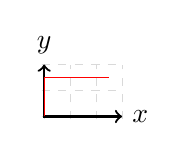
\begin{tikzpicture}[scale=0.33]
    % Draw axes
    \draw[help lines, color=gray!30, dashed] (-0.1,-0.1) grid (3.0,2.0);
    \draw [<->,thick] (0,2) node (a) [above] {$y$}
        |- (3,0) node (b) [right] {$x$};
    % Draw two intersecting lines
    \draw[color=red] (0,0) -- (0,1.5) coordinate (b_1) -- (2.5,1.5) coordinate (b_2);
\end{tikzpicture}
\qquad
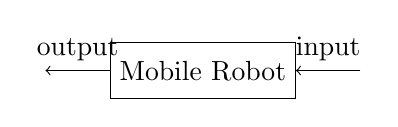
\begin{tikzpicture}[node distance=2.5cm,auto]
    \node [draw, minimum size=2em] (a) {Mobile Robot};
    \node (b) [right of=a,node distance=2cm, coordinate] {a};
    \node (c) [left of=a,node distance=2cm, coordinate] {a};
    \path[->, above] (b) edge node {input} (a);
    \path[<-, above] (c) edge node {output} (a);
\end{tikzpicture}
\qquad
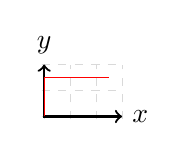
\begin{tikzpicture}[scale=0.33]
    % Draw axes
    \draw[help lines, color=gray!30, dashed] (-0.1,-0.1) grid (3.0,2.0);
    \draw [<->,thick] (0,2) node (a) [above] {$y$}
        |- (3,0) node (b) [right] {$x$};
    % Draw two intersecting lines
    \draw[color=red] (0,0) -- (0,1.5) coordinate (b_1) -- (2.5,1.5) coordinate (b_2);
\end{tikzpicture}



\end{document}